
%%%%%%%%%%%%%%%%%%%%%%%%%%%%%%%%%%%%%%%%%%%%%%%%%%%%%%%%%%%%%%%%%%%%%%%%%%%
%
% Plantilla para un artculo en LaTeX en espaol.
%
%%%%%%%%%%%%%%%%%%%%%%%%%%%%%%%%%%%%%%%%%%%%%%%%%%%%%%%%%%%%%%%%%%%%%%%%%%%

\documentclass[11pt,twoside]{report}

% Esto es para poder escribir acentos directamente:
%\usepackage[latin1]{inputenc}
\usepackage[utf8]{inputenc}
\usepackage{makeidx}
\usepackage{multirow}
\usepackage{titlesec}
\usepackage{sectsty}
\usepackage{fncychap}
\usepackage{color}

% Esto es para que el LaTeX sepa que el texto est en espaol:
\usepackage[spanish]{babel}
\usepackage[right=3cm,left=3cm,top=2.5cm,bottom=2.5cm,headsep=1cm,footskip=2cm]{geometry}
\usepackage{graphicx}
% Paquetes de la AMS:
\usepackage{amsmath, amsthm, amsfonts}

%\pagestyle{headings}
\pagestyle{myheadings}
\markboth{Informe Semanal de Actividades Realizadas}{Informe Semanal de Actividades Realizadas}
\begin{document}
\title{\color{red}Informe Semanal de Actvividades Realizadas}
\author{Nombre: Arturo Veras\\ 
Supervisor: Claudio Torres\\
Empresa: CCTAVAL\\
Tipo de Práctica: Profesional}
%\date{\color{green}December 2005}
\maketitle
%\setlength{\unitlength}{1 cm} %Especificar unidad de trabajo
\thispagestyle{empty}
\begin{picture}(0,1.5)
\put(0,0){
\includegraphics[width=2.7cm,height=2cm]{utfsm.jpg}}
\put(13,0){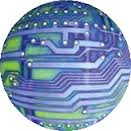
\includegraphics[width=2cm,height=2cm]{elo.jpg}}
\end{picture}
\\
\\
\begin{center}
\textbf{{\LARGE Universidad Técnica Federico Santa María}\\[0.5cm]
{\LARGE Departamento de Electrónica}}\\[4.25cm]
{\Large Informe de Práctica}\\[2.3cm]
{\LARGE \textbf{Centro Cient\'ifico Tecnol\'ogico de Valpara\'iso}}\\[3.5cm]
{\large Arturo Veras Olivos}\\[2cm]
Valparaiso - \today
\\
 {\large Versión 2.5}
\end{center}

%\newpage
%\tableofcontents
%\listoffigures % to produce list of figures
%\listoftables % to produce list of tables
%\newpage
\subsection*{Semana 1,  del $13/01/14$ al $17/01/14$}

El trabajo principal se centra en conectar una GPU (Graphic Card Unit) a una
Raspberry Pi (le llamaremos RPi desde ahora), específicamente se quiere
conectar una GT640 la cual tiene una interfaz PCIe 3.0 16x. Cabe destacar que
usar una Rpi no es primordial, es posible que dentro de la investigación se
encuentre una tarjeta que funcione mejor.  La RPi tiene dos interfaces que
estan disponibles para la conexión: (1) el puerto GPIO (General-Purpose
Input/Output) y (2) el puerto USB 2.0 los cuales tendremos que investigar si
sirven para nuestro propósito.  Para realizar la conexión se plantearon las
siguientes ideas:

Se propuso utilizar la tarjeta de desarrollo startKIT, esta tarjeta
particularmente posee una interfaz PCIe  1x la cual podemos utilizar.  Se
propone esta idea porque la tarjeta startKIT se conecta fácilmente a la Rpi a
travs del puerto GPIO.  Esta idea fue descartada porque los drivers de la
interfaz PCIe solo existen para las sliceCARD, estas son tarjetas diseñas
(WIFI, audio, etc.) especialmente para la startKIT. Para conectar la GPU
debemos desarrollar nuestro propio controlador, el que no podemos realizar
debido al limitado tiempo del proyecto.  

La otra idea que surgió fue la de estudiar los adaptadores de PCIe a USB. Estos
utilizan un chip para realizar la tarea el cual, eventualmente, podríamos
utilizar y diseñar una placa para que cumpla nuestros requerimientos, es decir,
conectar la tarjeta PCIe 16x al puerto USB 2.0. Se encontró el chip MCS9901-CC
que es el encargado de realizar el puente entre estas interfaces.  

Una tercera idea es usar un adaptador PCIe a mPCIe llamado PE4L-PM060.  La idea
tras este adaptador es utilizarlo en caso de que se utilice una alternativa a
la Rpi que tenga un puerto mPCIe lo cual es más facil de encontrar en el
mercado.  Esta alternativa tambin fue descartada porque no cumple los
requerimientos. Se encontró un dispositivo que potencialmente puede realizar lo
que necesitamos. 



The FBFPE4L-PM0FBF60A is a PCIe Adapter. The PE4L is designed for Notebook PCs that
converts PCI Express 1X add-on Card to ExpressCard or mPCIe connecter or PCI
Express slot. As PCI Express x1 connector is edge-free / multi-lane, x4, x8 and
x16 PCIe Cards are also available. This adapter allows you to use your existing
PCI-E 1X Card in the notebook PC or Desktop PC for test. or AD-DC12V adapter).
The RPi doesn't have a mPCIe interface so this adapter would be an option in
the case of changing the RPi for another embedded system with MPCIe interface.

\subsection*{Semana 2, del 20/01/14 al 24/01/14}

Las tareas de esta semana consisten en seguir buscando otras alternativas ya que las
anteriores han sido descartas por el momento.

El chip USB2380 es un controlador PCIe 1.0 a USB 2.0. El problema es que tenemos que
desarrollar una tarjeta y realizar el driver. Es posible pero escapa de nuestros
conocimientos en estos momentos, se necesita más investigación y estudio para realizar
este tipo de trabajos, además requiere tiempo. 

Como no se ha encontrado un adaptador directo entre PCIe y USB se decide por estudiar la
posibilidad de realizar una tarjeta que tenga ambas interfaces y que cumpla con nuestros
requerimientos. Las posibilidades son : \textbf{MCS990} PCIe to 4-Port USB 2.0 Host
Controller y \textbf{USB2380} PCIe 1.0 to USB 2.0 controller.


The GT640 has a PCIe 3.0 16x interface, the host controllers support PCIe 1.1. In PCIe there is no problems with the connectivity with older versions. To connect the GT640 we need a PCIe 1x to 16x Powered Flexible Riser. In theory we have all we need to build a prototype that does the job. The next question is if the GT640 is going to be recognized by the RPi, there is driver support for this application? can we use the existing legacy drivers or we have to implement a new one?

In the meanwhile we are in contacts with the vendors to to see what they say about the feasibility of the project.

January Wednesday 22

Some of the vendors respond to our emails but the did't understand the requirements that we need. We explained and still we are waiting for the response.

We are studying MCS9990. There is an schematic circuit to make the board, but this is not what we need. Therefore we need to make a deep study of PCIe protocol and the MCS9990 chip to develop the PCIe to USB 2.0 adapter. This option is out of discussion because the time consuming of developing time is very high.

In conclusion any attempt to create an interface using a chip is discarded.

January Thursday 23

The SBC-A510 Single Board Computer. is a mini-ATX compliant, single board computer. Important features:

Single board computer implemented by the combination of a CM-A510 module and a SB-A510 baseboard. Mini-ATX form factor.
1GB DDR3
PCI Express and PCI extension interfaces
The price for 1k unit: USD $65. For 1 quantity 2.5*$65 = USD $163
January Friday 24

We couldn't find a definitely solution to the problem. This is the summary so far:

Found a USB 2380 board that can we use but the vendor did not contact us yet.
Use the PE4L-PM060A in the case of acquiring a board with the mPCIe.
Completely ruled out the solution to implement the MCS9990 chip or similar, not a feasible solution.
The project will take another tack. Since we can not, for the moment, to find a solution to connect the RPI to a PCI card, the new approach will be to seek ways to connect the GPU to some device that that we can transfer data through an USB port. The options we have high to low priority.

Development boards with PCIe slot that we can buy this week or soon.
mPCIe to PCIe adapter so we can use the development board that we already have.
Build a cheap computer to use as PCIe interface.
Finally we decided to use the USB port to communicate with the GPU to make a Plug and Play device. There can be another ideas like use the Ethernet port but the USB is going to be the main work. So, we need to find solutions to the problem of connecting the Host PC to the RPi or some other device which in turn will be connected to the GPU.
\subsection*{Semana 3, del 27/01/14 al 31/01/14}
\subsection*{Semana , del 03/02/14 al 07/02/14}



\end{document}
